\chapter{Estado de la Cuestión}
\label{cap:estadoDeLaCuestion}

Actualmente Internet aloja una cantidad ingente de información de todo tipo. A pesar de los beneficios evidentes que supone tener tanta información subida a la web, este hecho también trae consigo problemas debido a dificultades semánticas, un más que elevado número de fuentes de información y el propio tamaño de los datos. Como consecuencia de esto, para poder hacer consultas a información y navegar de un contenido a otro que esté conectado es necesario tener un sistema de organización para toda esa cantidad de datos.\\

A continuación exponemos tecnologías cuyo objetivo es acceder a datos con un contexto y a facilitar el proceso de búsqueda al proveer información verdaderamente relevante para los usuarios.\\

\section{Conceptos sobre el ámbito}

La llamada \textbf{Web Semántica} es una extensión de la World Wide Web propuesta por Tim Berners-Lee \cite{berners2001}, cuyo objetivo es proveer a los datos estructura y significado. Con esto se consigue que la información de la web sea más fácilmente comprensible para las máquinas (o agentes de software). De esta forma se desea lograr que los agentes no solo analicen gramaticalmente, sino que comprendan la gran cantidad de información contenida en la web. 


Actualmente un navegador puede ejecutar una búsqueda de una palabra en la web de forma que el resultado que obtendremos será producto del análisis de los caracteres de nuetra palabra, es decir buscará una serie de documentos que contengan esa cadena de caracteres. Sin embargo el concepto principal de la Web semántica es que todas estás búsquedas relacionen conceptos perecidos a lo que refiere esa palabra. Esa búsqueda de conceptos no tiene por qué coincidir con la sintaxis de la palabra buscada si no con sus diferentes significados. De esta forma no nos limitamos a una búsqueda simple si no que muchos conceptos de distintos contextos son relacionados dotando de una mínima inteligencia a un sistema\cite{CODINA, Lluís; ROVIRA, Cristòfol. La web semántica. En Tendencias en documentación digital. Trea, 2006.}.\\

Gracias a este entendimiento, los agentes podrán integrar datos de diversas fuentes, inferir hechos ocultos y responder a consultas complejas fácilmente. Finalmente lo que se ha creado es un sistema que permite navegar por la información mediante enlaces o hipervínculos, navegando así entre datos conectados \cite{sakr2018}.\\

Para poder hacer realidad esta Web Semántica es necesario que la información de la web sea accesible en un formato estandarizado, accesible y manejable por las herramientas de la Web Semántica. Además, no basta con tener acceso a los datos sino también a la relación entre la información, lo cual marca la diferencia entre la Web Semántica y una simple colección de datasets. Esta colección de datos interrelacionados es lo que llamamos \textbf{Linked Data} (o datos enlazados) y será la base de nuestro trabajo en el dominio de los temas musicales.\\


Para poder hacer realidad esta Web Semántica es necesario que la información de la web sea accesible en un formato estandarizado, accesible y manejable por las herramientas de la Web Semántica. Además, no basta con tener acceso a los datos sino también a la relación entre la información, lo cual marca la diferencia entre la Web Semántica y una simple colección de datasets. Esta colección de datos interrelacionados es lo que llamamos \textbf{Linked Data} (o datos enlazados) y será la base de nuestro trabajo en el dominio de los temas musicales. Normalmente cuando queremos referenciar una página web o un documento, tenemos un identificador único que simplemente nos proporciona un acceso al sitio web pero no nos da opción a saber nada más de el. El pricipal motor o sentido del concepto de linked data es poder acceder a un documento pero también poder dotarlo de un concepto o significado para depués poder referenciar otros documentos con este mismo concepto. \\

Hay dos tecnologías que sirven como modelo a la hora de configurar y organizar toda esta información. La primera es el modelo XML ``Standard Generalised Mark-up Language''. Este sistema se basa en la utilización de etiquetas para la descripción y organización de los datos. Un documento XML es capaz de marcar y dotar de significado diferentes partes de un texto que se necesiten nivelar o etiquetar. Se utilizar tanto para representar información en una página HTML hasta organizar registros de una base de datos. \cite{Tom Heath; Christian Bizer, "Linked Data: Evolving the Web into a Global Data Space," in Linked Data: Evolving the Web into a Global Data Space , Morgan & Claypool, 2011.} \\

El segundo sistema estructural y actualmente el que nos interesa para este proyecto es el \textbf{Esquema RDF} (Resource Description Framework), que es un modelo de datos basado en declaraciones sobre recursos web mediante expresiones sujeto-predicado-objeto. Dichas expresiones se llaman ``tripletas'', donde el sujeto representa al recurso, el objeto representa el valor del recurso y el predicado supone los rasgos o aspectos del recurso que relacionan sujeto y objeto \cite{sakr2018}. Un ejemplo a grandes rasgos podría ser el siguiente:\\

:Juan es :Persona

:Juan hijoDe :María\\

Con este simple ejemplo ya hemos representado el hecho de que existe algo llamado Juan, que es una persona y además es hijo de María. Aquí hemos juntado dos conjuntos de tuplas o tripletas relacionadas entre ellas de una forma que podemos representar mediante un grafo.\\

Es necesario señalar que este es un ejemplo muy básico y sencillo. En la web real, existen millones de tripletas relacionadas entre sí por lo que en nuestro ejemplo tanto juan como María tendrían un número muy alto de tripletas más que representan toda la información que se tiene sobre ellos en la web.\\

A la hora de llevar esta explicación a un nivel más técnico y realista, estas expresiones no se formulan con sus nombres en lenguaje natural que hemos usado para el ejemplo. Estos tres argumentos que conforman la unidad de tripleta, se representan mediante un Identificador de Recursos: una URI~(Uniform Resource Identifier) \cite{sakr2018,berners2007}.\\

Una URI~(Uniform Resource Identifier) es una cadena de caracteres que puede identificar una entidad o recurso por su nombre o bien por su ubicación, la cual muestra dónde podemos acceder a él. Siguiendo esta división, una URI puede comprender el URL~(Uniform Resource Locator) y el URN~(Uniform Resource Name). La URN identifica la entidad por su nombre, lo cual no nos proporciona su ubicación y no asegura que esta entidad esté disponible. Sin embargo, la URL nos proporciona la localización directa de la entidad y esta es la principal razón de que sea mucho más usada en la web \cite{berners1994,saint2017,sakr2018}.\\

Volviendo a lo que respecta al modelo RDF, hemos determinado el hecho de que si empleamos este lenguaje seremos capaces de relacionar un sujeto y un objeto mediante un predicado, de forma que obtendremos un grafo similar al de la Figura 2.1.\\

\begin{figure}[h!]
	\centering
	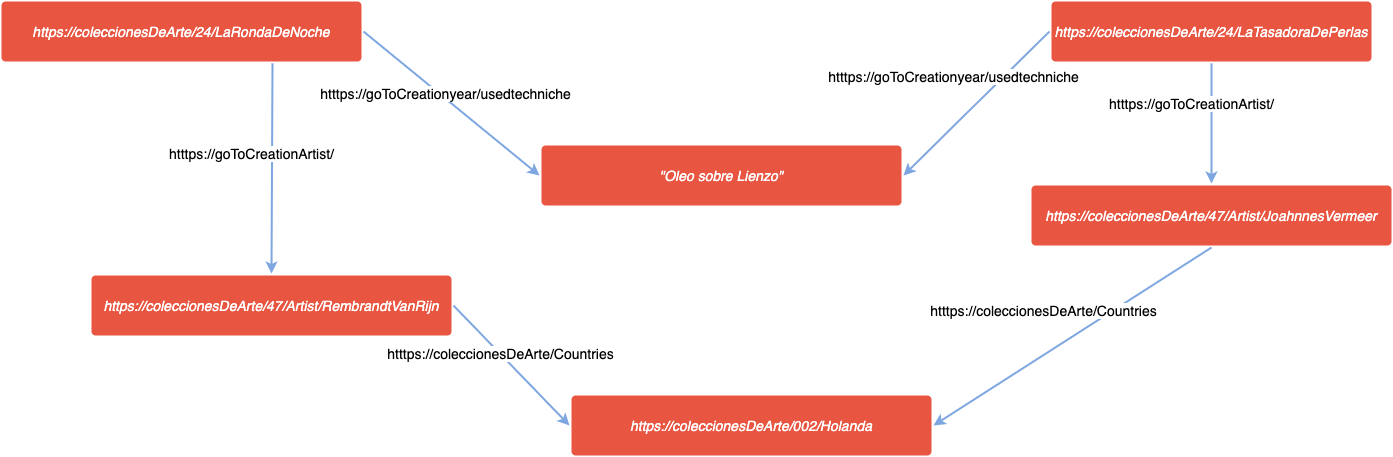
\includegraphics[width = 1\textwidth]{Imagenes/Bitmap/RDFexample.png}
	\caption{Ejemplo de grafo siguiendo el modelo RDF}
	\label{fig:sampleImage}
\end{figure}

Para una persona normal, esta puede resultar una nomenclatura poco amigable ya que las URIs pueden llegar a ser mucho más engorrosas y complejas. Más adelante explicaremos cómo hemos resuelto este problema en nuestro proyecto para que cualquiera que haga uso de nuestra interfaz pueda reconocer todos los objetos y, sobre todo, para darnos mucha más comodidad a la hora de trabajar con ellos.\\

Podríamos decir que estamos estableciendo una relación entre dos objetos unidos mediante una propiedad. Esta propiedad es una ``explicación'' que nos sirve para relacionar objetos. En nuestro proyecto, estos objetos son canciones.\\


\section{Herramientas con uso de Linked Data}


\section{SPARQL}

Finalmente, para poder empezar a trabajar con la información hemos usado el lenguaje SPARQL, el cual nos permite consultar los datos enlazados de la web. Este es un lenguaje especializado para buscar y consultar datos RDF. Básicamente facilita el acceso a las URIs para después poder aplicar todo tipo de selección de datos, restricciones, condiciones y límites a las entidades con los esquemas explicados anteriormente. La estructura de una consulta SPARQL suele ser la siguiente:\\

\begin{lstlisting}[language=SPARQL]
PREFIX EX: Uri de una web
SELECT * variables que se desean conseguir
WHERE
{
	Operaciones con tripletas
}
OFFSET X intervalo de desplazamiento
LIMIT X limite de los datos obtenidos
\end{lstlisting}
\bigskip

La cadena PREFIX hace referencia a la URI o URIs donde se encuentran localizados las entidades a las que hacen referencia las tripletas. Su objetivo es no tener que escribir la URI entera, la cual es una cadena de texto poco amigable para un usuario, cada vez que lo referenciáramos en una relación de las tripleta dentro de la cláusula WHERE.\\

A la hora de hacer una consulta compleja, es posible que lleguemos a un código que referencie muchas URIs y entidades de forma que no sea un lenguaje de uso fácil. Es por esto por lo que pudimos encontrar variedad mediante la librería que nos dispone Wikidata que simplifica algo más la nomenclatura y los caracteres de este lenguaje.\\

\section{WikiData}

Wikidata es una base de datos libre, colaborativa, multilingüe y secundaria, que recopila datos estructurados para dar soporte a Wikipedia, Wikimedia Commons, así como a otras wikis del movimiento Wikimedia y a cualquier persona en el mundo \cite{wikidataIntro}. El proyecto comenzó en 2012 liderado por Wikimedia Alemania. Gracias a Wikidata, tenemos una gran cantidad de información relevante acerca de toda nuestra cultura reunida en un mismo sitio. La usaremos para consultar e investigar la información relacionada con nuestro dataset (o conjunto de datos), esencialmente datos acerca de artistas y sus temas musicales. Tiene numerosos servicios, uno de los que probablemente hayamos usado y no nos hemos dado cuenta, es el de servir información para rellenar las fichas de los artículos de Wikipedia.\\

Wikidata está estructurada de tal manera que resulta sencillo acceder a su información utilizando el lenguaje de consultas SPARQL. Cada objeto tiene ciertas propiedades a las que podemos acceder seleccionando el identificador correcto de la propiedad.\\

Una de las ventajas de Wikidata es que nos va a eliminar toda la nomenclatura de URIs propias de SPARQL. En estas consultas, las entidades serán referenciadas con los caracteres wd y las propiedades con los caracteres wdt. Un ejemplo de una consulta sencilla podría ser:\\

-Obtén todos los Artistas cuyo género musical sea Rock:\\
\begin{lstlisting}[language=SPARQL]
SELECT ?singer ?singerLabel ?genre ?genreLabel
WHERE
{
	?singer wdt:P31 wd:Q215380;
	wdt:P136 wd:Q7749;
	SERVICE wikibase:label { bd:serviceParam wikibase:language &quot;en&quot; . }
}
\end{lstlisting}
\bigskip

En esta consulta estamos accediendo a todos los objetos que contengan las propiedades~(wdt) P31~(Tipo Instancia) y P136~(Género) con el valor~(wd) que nosotros estamos seleccionando, Q215380 y Q7749, forzando así a que las dos propiedades sean Grupo Musical y Rock and Roll respectivamente.\\

SPARQL es un lenguaje muy potente que puede abarcar gran cantidad de datos en función de la web (se pueden crear consultas mucho más complejas para obtener datos más específicos).
